\documentclass{ledger}

%AUTHOR: This is a bare-bones template into which you may put your paper to aid in formatting your submission to Ledger. Note that to work properly, you must have the files "ledger.cls", "ledgerbib.bst", and the folder "images" on hand. 

%AUTHOR: the preferred method to generate PDF output is to use 'pdflatex'
%To clean up after a successful build, try: 'latexmk -c main.tex'


%EDITOR: replace X's to set the data for the header and footer
\newcommand{\thefirstpagenum}[0]{X}
\newcommand{\thelastpagenum}[0]{X}
\newcommand{\theyear}[0]{20XX}
\newcommand{\thevol}[0]{X}
\newcommand{\thedoi}[0]{DOI 10.5195/LEDGER.\theyear.XXX}
\newcommand{\ledgerpages}[0]{\thefirstpagenum-\thelastpagenum}


%AUTHOR: please set these to generate correct PDF metadata
\hypersetup{pdfauthor={PredictChain}, pdftitle={PredictChain}}

%EDITOR: set the correct pageination during layout
%\setcounter{page}{\thefirstpagenum}


%AUTHOR: this can be used to highlight changed text, surround with \edit{} and
%uncomment either to determine color
%\newcommand{\edit}[1]{{\color{red} #1}}
\newcommand{\edit}[1]{#1}
	
\overfullrule=10pt

\title{PredictChain:\\
A Blockchain-based Predictive Marketplace}
\author{
    MTP
    CJP
}

\pagestyle{pagemain}


%The Author should select the appropriate pretitle below:
\pretitle{
  %\centering \selectfont LEDGER \LaTeX \ TEMPLATE \par
  %\centering \selectfont REVIEW ARTICLE \par
  \centering \selectfont RESEARCH ARTICLE \par 
  \fontsize{24pt}{28pt}\selectfont} % Title is centered and at 24pt


\begin{document}

\maketitle

\thispagestyle{pagefirst}

\begin{abstract}
One of the main issues with artificial intelligence training and development today is accessibility. Oftentimes,
individuals or groups possess data that they would wish to be used in predictive analysis. However, these people
may not have access to the compute capacity to train predictive models on this data.  Additionally,yet other
people have neither access to predictive training data, nor do they have access to adequate computational resources.
Compounding this issue is the fact that the entities that \textit{do} have these computational resources often keep the results of
trained models hidden from the public.  Due to this lack of accessibility, similar models are often trained on similar datasets,
obtaining similar results.  This results in both a notable inefficiency, and the withholding of useful predictions from
the majority of people.

To help to aid with this issue, we propose PredictChain, a blockchain-based marketplace for predictive AI models.
Through PredictChain, users are able to upload datasets for training predictive models, request that train models
be trained on any previously uploaded datasets, or submit queries to those trained models.
These various models will be operated by a central node or nodes with computing resources available. A variety of
models will be made available, ranging from cheap, fast, and simple to more expensive, slower, and more powerful.
This will allow for a large variety of predictive abilities for both simple and complex patterns.  All the past predictions
form these models will be stored on the blockchain for public viewing.

Given enough users, this project would have a notable impact on the state of machine learning usage.  Currently,
the problem of accessibility prevents many people from utilizing machine learning themselves, often leaving them to
turn to highly private and centralized tech giants.  This project would serve to open up this black-box of
an industry and encourage the sharing of datasets and parameter configurations to create better models that are open
to the public for usage.

%AUTHOR: keywords are OK to show for Review article, will be hidden and added to metadata for publication
\begin{keywords}
\item Bockchain.
\item Decentralized.
\item Marketplace.
\item Oracle.
\item LSTM.
\item GRU.
\item RNN.
\end{keywords}
\end{abstract}

\pagebreak

\section{Project Description}

\subsection{Problem Solved}

PredictChain helps to solve one of the main issues that involve AI models today: accessibility.  Our project fulfils this
need in two ways.  Oftentimes, individuals or groups poses data that they would wish to be used in predictive analysis.
However, these people may not have access to the compute capacity needed to train predictive models on this data.  Additionally,
yet other people have neither access to predictive training data, nor do they have access to computational resources.
PredictChain solves both of these problems simultaneously.

When users upload their datasets, they allow a model to be trained on those datasets.  Higher quality datasets will produce
higher quality models.  When users submit parameters for training, they allow the model that their parameters produce to
be used publicly.  Both of these users are rewarded for their work when a model is queried.  The amount of this reward
is based off of the correctness of the prediction.  This encourages users to participate in contributing the
resources needed for good predictions, while leaving a public record for other users to view.

\subsection{Significance}


As the trend of ever-growing machine learning models continues, this problem becomes increasingly relevant.
As the scale and power of these models grow, the resources required to train them grow as well.  This makes the training
of useful machine learning models unattainable for most people.  In order to get useful results from these models,
users often have to pay large, centralized organizations, without any reward if they provide a good dataset or model
parameters.  PredictChain changes this paradigm by incentiveizing the thoughtful creation of useful models and
datasets.

Additionally, after the recent mania and subsequent crash around blockchain adjacent technologies, it has become
important to remind people that blockchains can be used for genuine utility in addition to investment.  By primarily
using Algos as a method of payment, instead of investment, it helps to, once again, show that cryptocurrencies can
effectively be used as a pure form of payment for useful services.  Of course, this is in addition to the many other
services that use crypto in a similar manner, but adding one more project only helps the Algorand's notion of usefulness.


\subsection{Use Cases and User Stories}

The following use cases and user stories demonstrate our target audience and several of the core components of PredictChain.

\paragraph{User Story \#1}
\textit{Scenario:} As a data analyst, I want to have access to trends of various stock markets so that I can create
predictive models that will inform my investment strategies.

\paragraph{User Story \#2}
\textit{Scenario:} As a stockbroker, I want to compare my dataset to another dataset while using the same model so that
I can get an idea as to which is better.

\paragraph{Use Cases}
For the sake of space, we will only go over two simple use cases; one that allows the user to add a dataset and
another where a user queries a prediction from an existing model.

\begin{table}[H]
    \caption{Add Dataset}
    \label{tab:add-ds}
    \centering
    \begin{tabular}{|p{3cm}|p{11cm}|}
        \hline
        \textbf{Identifier:} & UC1 \\
        \hline
        \textbf{Description:} & The user logs in to PredictChain and adds a dataset to their account\\
        \hline
        \textbf{Actor(s):} & Site User \\
        \hline
        \textbf{Precondition(s):} & The user has a publicly available link for the dataset\\
        \hline
        \textbf{Event Flow:} &
        \begin{enumerate}
            \item The user logs in properly into their account (or creates a new account)
            \item The user checks to see how much it would cost to upload a dataset, given the size of the dataset
            \item The user inputs a link to the dataset file in the upload dataset area
            \item The user inputs a name corresponding to that dataset
            \item The user enters in the size of the dataset file in bytes
            \item The user presses "Submit"
        \end{enumerate} \\
        \hline
        \textbf{Postcondition(s):} &
        \begin{enumerate}
            \item A dataset has been created and is stored in the oracle
            \item The transaction has been stored on the blockchain
            \item The website displays the information onto the dashboard corresponding to the outcome
        \end{enumerate}\\
        \hline
    \end{tabular}
\end{table}

\begin{table}[H]
    \caption{Model Query}
    \label{tab:model-query}
    \centering
    \begin{tabular}{|p{3cm}|p{11cm}|}
        \hline
        \textbf{Identifier:} & UC2 \\
        \hline
        \textbf{Description:} & The user logs in to PredictChain and queries a prediction from an existing model\\
        \hline
        \textbf{Actor(s):} & Site User \\
        \hline
        \textbf{Precondition(s):} & The user is ready with information concerning the model training parameters \\
        \hline
        \textbf{Event Flow:} &
        \begin{enumerate}
            \item The user logs in properly into their account (or creates a new account)
            \item The user selects an existing model from the dropdown under the query model area
            \item The user inputs a list of numbers corresponding to the input data of the model
            \item The user submits their request using the submission button in that section
        \end{enumerate} \\
        \hline
        \textbf{Postcondition(s):} &
        \begin{enumerate}
            \item The website displays the result of the query onto the dashboard
            \item The result of the query is stored on the blockchain
        \end{enumerate}\\
        \hline
    \end{tabular}
\end{table}

\section{Implementation Details}

The structure of PredictChain is primarily broken up into two parts: the client and the oracle.  Both of these parts
interact with each other through the blockchain.  The following diagram illustrates this relation:

\begin{figure}[H]
    \begin{center}
        \begin{minipage}{0.6\textwidth}
        \centering
        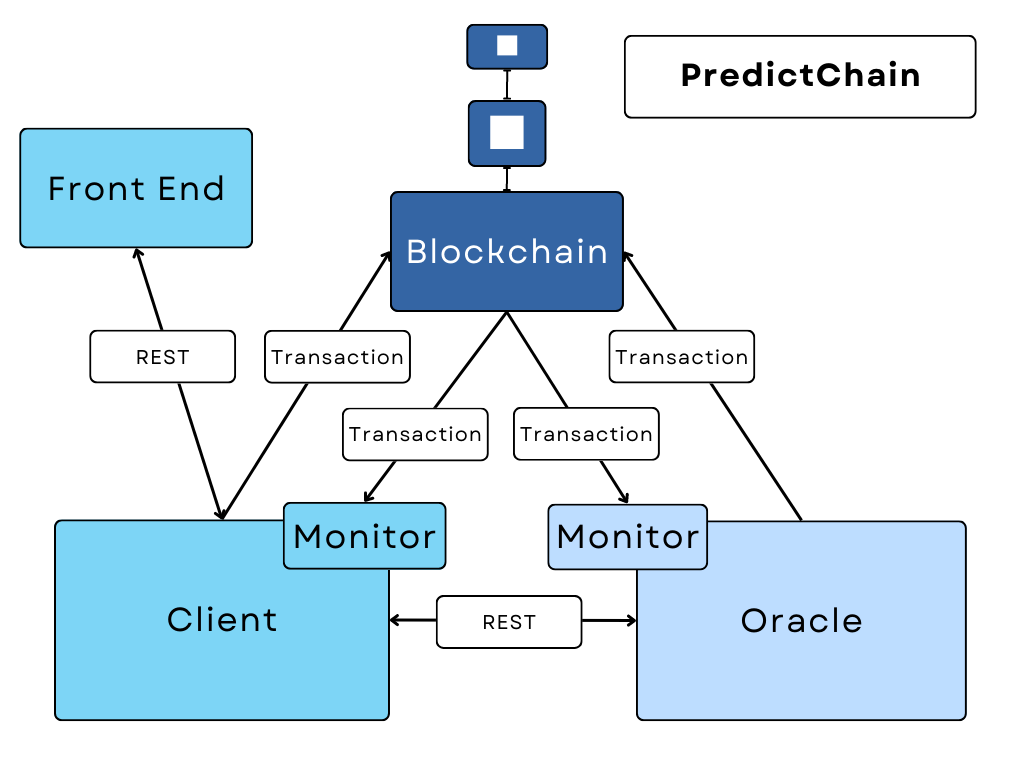
\includegraphics[width=\linewidth]{images/detailedDiagram}
        \caption{The architecture of PredictChain}\label{Fig:detailedDiagram}
    \end{minipage}\hfill
    \end{center}
\end{figure}

The above diagram illustrates the core components of the system, along with their methods of communication.

\subsection{The Front End UI}
Although not directly related to the AI or the blockchain parts of the product, it is still important to discuss the
UI aspect of our project. The UI sets the user's impression of PredictChain by having multiple pages that create a more
pleasant experience for the user. For example, the home page talks about our mission, how we differ from our
competitors and example model sets we provide. The addition of the \textit{FAQ} and \textit{Meet the Team} pages allow users to
understand who created PredictChain, as well as get answers about any privacy/security concerns they might have.
Lastly, users can create an account or login to a pre-existing account. Then users are able to use PredictChain
to its fullest functionality such as adding datasets, checking prices, or querying models with provided datasets.
The UI talks to the client through a series of REST requests in order to convey this data, later receiving the
result of the user's actions later through the same means.

\subsection{The Client}

The client serves as a middleman between the front end user interface and the blockchain.  It is run as a server,
serving UI content to the user, taking in requests from the UI, and parsing those requests into a form suitable for
both the blockchain and for the oracle.  Additionally, the client constantly polls for updates coming from the oracle,
through the blockchain, and then through its monitor.  These updates are queued and sent to the front end upon request.
This allows the user to both interact with the blockchain and to see the important updates that come from it.

\subsection{The Oracle}

\begin{figure}[H]
    \begin{center}
        \begin{minipage}{0.6\textwidth}
        \centering
        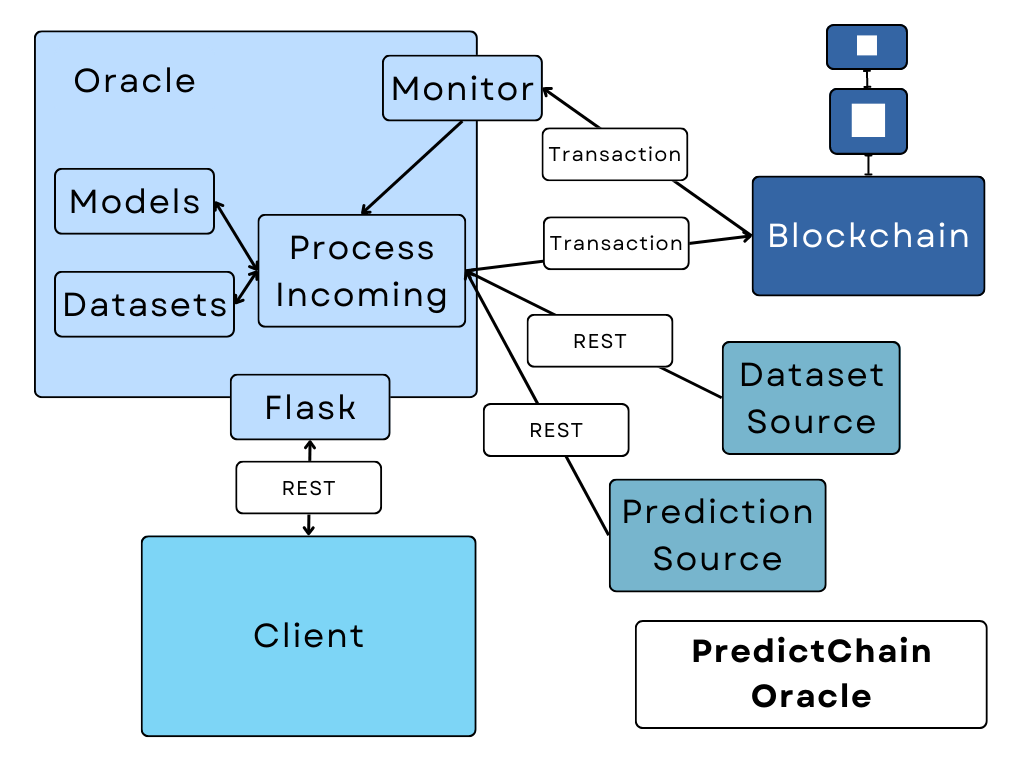
\includegraphics[width=\linewidth]{images/oracleDiagram}
        \caption{The architecture of the Oracle}\label{Fig:oracleDiagram}
    \end{minipage}\hfill
    \end{center}
\end{figure}

The oracle accomplishes the majority of the other tasks that this project requires.  It constantly polls for updates
coming from the client, through the blockchain by using its own monitor.  Upon receiving these updates, it begins
the execution of one of its three main operations.  These are:

\begin{itemize}
    \item Downloading a user-specified dataset and saving it
    \item Training one of the raw models based on user inputted parameters
    \item Querying one of the trained models on user inputted data and comparing it to the real-world result
\end{itemize}

After each of these operations, the oracle sends out several blockchain transactions.  These can be either
rewards to contributors of a model or confirmations/results of the operation that has been performed.

When working with user-submitted datasets, the oracle uses a handler to manage the operations performed on that dataset.
The handler can save datasets to a specified environment, load datasets from a specified environment, parse that dataset
as a pandas dataframe, and split the dataset by the values of one of its attributes.  The environments that the handler
recognizes are \textit{local} and \textit{IPFS}.  When using either of these environments, the handler abstracts away the
complexities of working with either of them into a unified interface.

When working with user-trained models, the oracle uses a similar, common interface.  This interface can create the model
architecture, train the model on a selected dataset, query the trained model, evaluate its performance, save the model,
and load it back from a specified environment.  When creating and training a model, the interface chooses among a group
of archetype or template models.  These models can be a:

\begin{itemize}
    \item Multi-layered perceptron neural network
    \item Recurrent neural network
    \item Long short-term memory neural network
    \item Gated recurrent unit neural network
\end{itemize}

Each of these models has a \textit{model\_complexity} attribute.  This is a simple float value, designed to give users
a general idea of how performant a model can be once trained and serves as a method of calculating the cost of using
or training that given model.  The attribute itself is calculated using the size of the network and a linear multiplier to
account for more complex model architectures.  For models like GRUs or LSTMs, the complexity is higher as they are more complex and often
better performing models.  For models like MLPs, the complexity is lower.  This gives the desired effect of faster, simpler
models being cheaper than the slower, more complex models without any heavy calculations.   The interface abstracts most
of the complexities of training, querying, and evaluating these models.  The only difference between them is the inclusion
of several optional parameters.

\subsection{The Blockchain}

In PredictChain, the blockchain serves as both a records keeper and a messenger between the client and the oracle.
This is accomplished by using transactions as a form of direct communication.  With every transaction sent, there is a note.
This note is a json-encoded string (encoded in base64) that communicates information about the operation that the transaction
is requesting and arguments for that operation.  These operations are represented by a series
of op codes.  These codes are abbreviations of the operation name enclosed in angle brackets, for example $\langle$\textit{QUERY\_MODEL}$\rangle$.
The arguments to these operations are represented as a named dictionary, with each key being the name of the argument and each
value being the argument itself.  This named strategy allows the program to be very flexible without worrying about the exact
ordering of the arguments.  Blockchain is quite useful in its role due to its immutability and its transparency.  Using
a blockchain means that all requests are permanently stored and public, so other users can see what type of models are useful
for specific datasets and what results those models have produced.

\subsection{Software and Libraries}

\subsubsection*{Python Libraries}

This project is primarily built in Python, using the Algorand SDK.  The SDK makes interacting with the blockchain
very straightforward.  Through the tools provided by this library, we can easily read and write transactions from
the Algorand blockchain.

Through Python, we also used data science and machine learning libraries such as Pandas
and Torch.  These libraries encapsulate many of the complexities of data preparation and model training for us.
By using these libraries, we were able to concentrate on the higher-level functions of the project instead of worrying
about the lower-level implementation.

Flask as also an important part of the project.  We used Flask to allow both
the client and oracle nodes to function as servers.  The client would take in requests from the user and send out
requests to the oracle.  The oracle would then take in those requests and issue responses.  We chose to use Flask in
client-oracle communication to cut down on the amount of trivial transactions that would otherwise be made.  For example,
it would not benefit the accessibility or transparency of the project greatly if the exchanged transactions were
dominated by simple '\textit{what is the price of \ldots}' requests.

\subsubsection*{Node Libraries}

Additionally, the front end utilizes the React framework and firebase.  React was useful to us as it streamlined the process of making
dynamic, modular code for the web interface.  Firebase was invaluable for handling administrative tasks such as keeping
track of registered users and their associated metadata.

\subsubsection*{Redis}

For the recommended configuration of the project, we use Redis as well.  Redis helps to provide a reliable store for
our metadata about models and datasets in a simple, persistent manner.

%\subsection{Resource Links}

%The following table will provide links to the various resources relevant to our project and its evaluation:

%\begin{table}[H]
%    \caption{{Project Resources}}
%    \label{tab:resources}
%    \centering
%    \begin{tabular}{|p{3cm}|p{11cm}|}
%        \hline
%        \textbf{Resource} & \textbf{Link}\\
%        \hline
%        GitHub & \href{https://github.com/AI-and-Blockchain/S23_PredictChain}{github.com/AI-and-Blockchain/S23\_PredictChain}\\
%        \hline
%        Python Documentation & \href{https://github.com/AI-and-Blockchain/S23\_PredictChain/blob/main/docs/sphinx/index.html}{
%        [Our GitHub]/docs/sphinx/index.html}\\
%        \hline
%        Overall Demo Video & \href{https://drive.google.com/file/d/1vv3BEMC5ru3oa1HLSEXGNvjdFcZbCas3/view?resourcekey}{drive.google.com/file/d/1vv3BEMC5ru3oa1HLSEXGNvjdFcZbCas3}\\
%        \hline
%        Technical Demo Video & \href{https://www.youtube.com/watch?v=icWc1qvhsgY}{www.youtube.com/watch?v=icWc1qvhsgY}\\
%        \hline
%    \end{tabular}
%\end{table}

\section{Evaluation}

While the most definitive evaluation would be to deploy our project and get feedback from actual users, we are limited
in our time and in our scope.  In place of this, we have devised several tests that are designed to evaluate each
component of the project on its own and how the entire project functions as a whole.

\subsection{Transactions}

The usage of transactions is central to the communications protocol of PredictChain, so making sure the protocol
functions correctly is critical to the evaluation of the project.  Thanks to the SDK, we had no issue with encoding the
notes and actually sending the transactions.  Where problems can potentially arise is within the
client and oracle monitors.

The monitors are classes inside the client and oracle that listen for any transactions that have their node address
as the recipient.  This listening is done using the Algorand indexer class and a constant polling for new transactions.
We noticed that this monitor would sometimes skip or duplicate incoming transactions.  As we developed fixes for
these issues, we constantly evaluated the performance of the monitor.  This was done through programmatically sending
one or more transactions to the client or oracle address and checking to see how the monitor handled them.  By comparing
the unique transaction ids of the sent transactions to those processed, we were able to evaluate the monitor,
identify issues, and create fixes. For example, we now constantly update the minimum timestamp the indexer can look
for transactions after and we also keep a registry of the ids of all past transactions.  This helps to eliminate
the duplicate transactions that were getting through.

\subsection{Models}

Another critical component of PredictChain is its usage of a variety of models.  At present, all of these models
are different types of neural networks.  However, these networks are not created equally, with each having different
qualities, architectures, and outputs.  In order to evaluate the performance of these models, we ran several experiments
on the models where their hyper-parameters and architectures were kept constant as they were tested.  For this
evaluation, we measured their performance on our sample dataset, The University of California, Irvine's \textit{Dow Jones
Index} data set~\cite{dowJones}.  This dataset has 16 different parameters, detailing the attributes of a range of
stocks from the first half of 2011.  For our usage, we do not eliminate any of these during training, although this
may be an opportunity for future improvement.  As for the models, they were all initialized with the following parameters:

\begin{table}[H]
    \begin{center}
        \caption{{Model Evaluation Parameters}}
        \label{tab:evalParams}
        \bgroup
        \def\arraystretch{1.2}
        \begin{tabular}{|p{4cm}|p{1cm}|p{8cm}|}
            \hline
            \textbf{Parameter Name} & \textbf{Value} & \textbf{Description}\\
            \hline
            \textit{epochs} & 70 & The number of epochs that the model would train for\\
            \hline
            \textit{target\_attrib} & \textit{close} & The attribute that the model was trying to predict, this is the daily closing price of the stock\\
            \hline
            \textit{hidden\_dim} & 5 & The number of neurons in each hidden layer\\
            \hline
            \textit{num\_hidden\_layers} & 1 & The number of hidden layers\\
            \hline
            \textit{time\_lag} & 0 & The number of time steps that pass between the input window and the prediction\\
            \hline
            \textit{training\_lookback} & 10 & The number of time steps that recurrent models receive as input\\
            \hline
            \textit{sub\_split\_value} & 0 & The integer id of the stock to predict, in this case its is \textit{\$AA} (Alcoa Corp)\\
            \hline
        \end{tabular}
        \egroup
    \end{center}
\end{table}

We performed this test on all of our basic model structures, specifically our GRU, LSTM, RNN, and MLP models.
In the following figures, we show the input data and predictions for each model.  We also show the final loss
and the final accuracy.  The loss is calculated using the mean absolute error function
$mae(x, y) = (\Sigma^n_{i=1} |y_i - x_i|) / n$ and our accuracy is calculated using
$acc(x, y) = \sigma(-mae(x, y)+e^2)$ where $\sigma$ is the sigmoid function.  Our accuracy function is modified
in this way so that very large losses are registered as somewhat accurate and lower losses are registered as
very accurate.  This helps to account for the very large losses generated by some of the less performant models.

The results of our evaluations are as follows:

\begin{figure}[H]
    \begin{minipage}{0.49\textwidth}
        \centering
        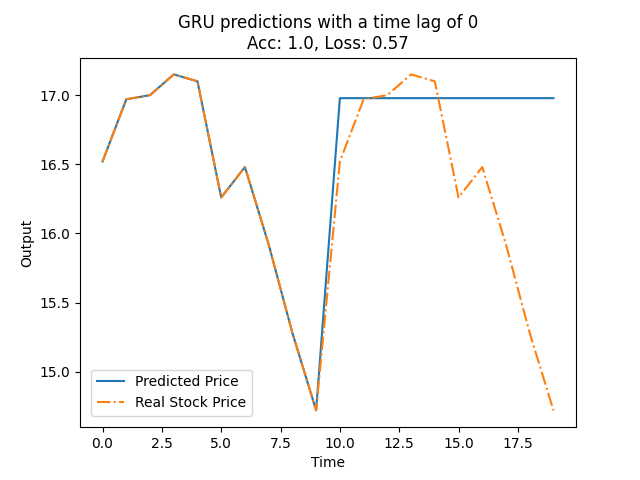
\includegraphics[width=\linewidth]{images/gruEval}
        \caption{The results from our GRU model}\label{Fig:gruEval}
    \end{minipage}\hfill
    \begin{minipage}{0.49\textwidth}
        \centering
        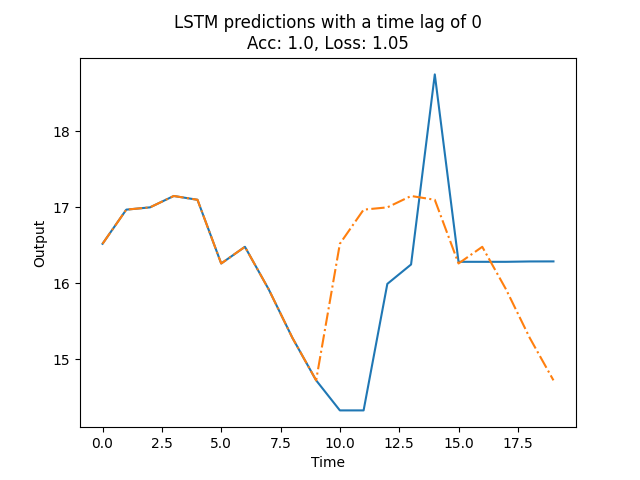
\includegraphics[width=\linewidth]{images/lstmEval}
        \caption{The results from our LSTM model}\label{Fig:lstmEval}
    \end{minipage}
\end{figure}

\begin{figure}[H]
    \begin{minipage}{0.49\textwidth}
        \centering
        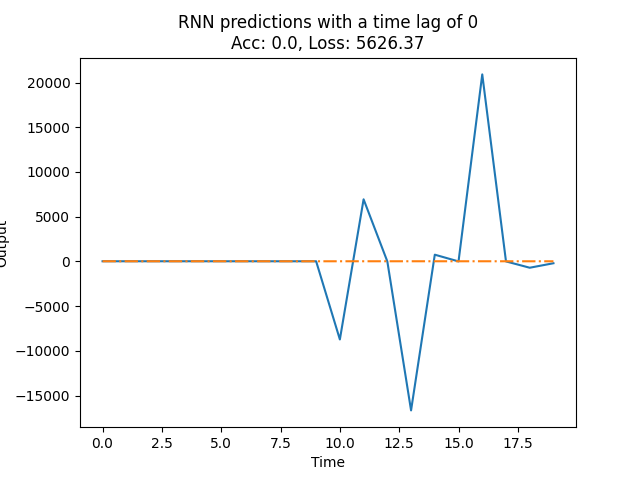
\includegraphics[width=\linewidth]{images/rnnEval}
        \caption{The results from our RNN model}\label{Fig:rnnEval}
    \end{minipage}\hfill
    \begin{minipage}{0.49\textwidth}
        \centering
        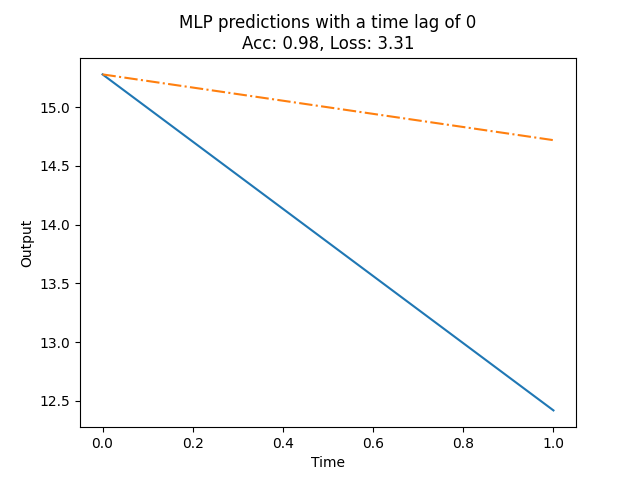
\includegraphics[width=\linewidth]{images/mlpEval}
        \caption{The results from our MLP model}\label{Fig:mlpEval}
    \end{minipage}
\end{figure}

Each of these results reflects the individual strengths and weaknesses of each model.  As is reflected in our
\textit{model\_complexity} calculations, the GRU model is the most performant, with a loss of only 0.57.  This is
closely followed by the LSTM model, which still offers a good prediction, but is slightly less consistent overall.
In our evaluation of our RNNs, we noticed a good example of the exploding gradients problem.  Without the limits
provided by the GRU and LSTM models, the predictions of the RNN become increasingly erratic.  Finally, our
MLP model does not suffer from an exploding gradient, but it does lack the recurrence of the other three models,
only being able to output one day at a time.

\subsection{End-To-End Testing}

The final component of our testing was the end-to-end series of tests we performed.  The goal of these tests was to
give us a holistic picture of how well our project functioned and how well that functioning met our stated goals.
For all of these tests, we started with front end user interaction and ended with the response to those actions.

\paragraph{Price Queries}
The first, and most straightforward, set of operations that we tested were the three price query operations.
We performed this test by submitting query requests on the front end, then tracing the functions called by that operation
from the client to the oracle, then to the oracle getting the price, then finally back to the client.  We performed
this test for all three of our queries, testing different sets of inputs, both valid and invalid, seeing if they
were handled properly.

\paragraph{Major Transactions}
The next set of tests we performed focused on our major transactions: \textit{Upload Dataset}, \textit{Train Model},
and \textit{Query Model}.  These tests were similar to those for the price queries.  As we performed these tests, we
noted that, while the operations did complete successfully, the user feedback and results were ambiguous.  Additionally,
we realized that it may be confusing for the user to remember the exact names of the models and datasets in order to
use them.  To address these issues, we made several additions.  To address the issue of users having to input the
exact names, we added a dropdown feature instead of a test input.  We now store a list of all current datasets and
models in the system.  This is updated upon the reloading of the page or when a user submits a transaction.  This
ensures the list is always updated for better ease of use.  To address the feedback issue, we added a feedback section
that periodically pinged the client to see if any new response transactions came in from the oracle.  If these
transactions did come in, we would display both the operation, the model or dataset name, and any extra data (like
the result of a query) to the user.  This way, the user would not have to manually check the transaction note on
the Algorand block explorer.

By performing these tests, we were able to both evaluate the quality of the project as a whole and make important
additions to improve the user experience.  Our transaction tests helped us to identify the issues that had
previously existed and to verify that the current communication protocol was working properly.  Our model tests
helped us to confirm our previous assumptions about the nature of our various models and which scenarios they are
most useful in.  Finally, our end-to-end testing confirmed the overall functioning of the project and inspired us
to make some valuable improvements to the user experience.

\section{Conclusion}

\subsection{Summary}

Over the course of our work, we have made PredictChain into a working blockchain-based marketplace for predictive AI models.
Through PredictChain, users are now able to upload datasets for training predictive models, request that basic models
be trained on any previously uploaded datasets, or submit queries to those trained models.
These various models will be operated by a central node with computing resources available. A variety of
models are available, ranging from cheap, fast, and simple to more expensive, slower, and more powerful.
This will allow for a large variety of predictive abilities for both simple and complex patterns.  All the past predictions
form these models will be stored on the blockchain for public viewing.

\subsection{Limitations}

A notable limitation that we experienced during this project were constraints on both our time and the amount of
hours we could each put into the project.  If this project was worked on for several months longer, the final product
would be significantly more fleshed out with more features.  If this were more akin to a multi-semester project,
we would have had the opportunity to add more starting datasets and add a more diverse set of models.

Another limitation that we had experienced was that we each had other commitments to other classes or activities.
This limited the amount of hours per week we could each work on improving the project.  To compensate for this, we
worked together to dynamically adjust our efforts by picking up the work of anyone that was unable to put as much
time into the project. This strategy helped us to stay on track while maintaining our prior commitments.

Despite, or perhaps aided by, these limitations, were able to budget our time and distribute the work in such a way
that out final project is in a functioning state that fulfils our initial objective: to create a prototype for a
accessible and transparent marketplace for machine learning training and predictions.

\subsection{Future Work}

As mentioned above, we have several opportunities for improvement that could be accomplished with future work
into this project.  One major improvement that we could make to the project is the overhaul of the architecture of
the project.  As mentioned previously, we had briefly considered using many model training nodes instead of a
centralized node.  Adding this would make the project more decentralized and open up another opportunity
for community contribution.  This would likely come in the form of users hosting training nodes and being rewarded for
the quality of models that it produces.  Another potential improvement that could be introduced with future work is
the addition of a greater variety of models or more example datasets.  Currently we only use neural networks to
use for predictions.  In future work, we would like to add a more diverse set of models, such as decision trees or
more statistical models based off of Bayesian inference.  Finally, we could make improvements to how our models are
trained, for instance, allowing users to prune off attributes from a dataset that they did not deem useful to the
trained model.  Adding these improvements may make PredictChain a more fleshed-out version of itself without changing
the core principles of our project.

\ledgernotes

\section*{Author Contributions}

MTP developed the bulk of the back end code, including the oracle, the client, the models, and the dataset management.
CJP worked, primarily, with the front end and user interface along with important contributions to client integration.

% \section*{Conflict of Interest}


%AUTHOR: comment out if using thebibliography
%\theendnotes

%AUTHOR: please read ledgerbib.bst usage notes by opening it in a text editor. We have modified it to include the use of the @misc item type for the proper formatting of online sources.

\bibliographystyle{ledgerbib}
\bibliography{main}

%AUTHOR: comment out, this is used to make sure the Creative Commons License
%image fits on page

%\newpage 	
%define the following sections to have the Appendix Style

%\appendix
%\setcounter{section}{0}
%\section{Data and Descriptions}

%\vspace{12pt}
%\begin{table}[h]
%\begin{center} 
%\scalebox{0.6}{ 
%\begin{tabular}{p{5cm}p{18cm}}%{l|}%{|>m{5cm}|>m{15cm}|}
%\rowcolor{orange}
%\hline
% \textbf{Column A}  & \textbf{Column B} \\\hline
%	Data & Description of data in more detail.\\
%\hline
 %Also Data & More description of data.\\
%\hline 
 %A Third Item & Pretium fusce id velit ut tortor pretium viverra suspendisse potenti. Enim sed faucibus turpis in eu. In hac habitasse %platea dictumst quisque sagittis. Pharetra et ultrices neque ornare aenean euismod elementum.\\
%\hline
%\hline
%\end{tabular}}
%\caption{A table in an appendix} \label{AppendixTable}
%\end{center}
%\end{table} 
%\newpage
%here up^^


\thispagestyle{pagelast}





%\theendnotes

\end{document}
